\documentclass[aps,superscriptaddress,prx,nofootinbib,twocolumn,truncate=10]{revtex4-2}
\usepackage{bm}
\usepackage{lmodern}
\renewcommand{\ttdefault}{lmodern}
\usepackage[utf8]{inputenc}
\setcounter{secnumdepth}{3}
\usepackage{amsmath}
\usepackage{amssymb}
\usepackage{upgreek}
\usepackage{graphicx}
\usepackage{epstopdf}
\usepackage[dvipsnames]{xcolor}
\usepackage{enumerate}
\usepackage{gensymb}
\usepackage{ulem}
\usepackage[T1]{fontenc}
\newcommand{\stkout}[1]{\ifmmode\text{\sout{\ensuremath{#1}}}\else\sout{#1}\fi}
\usepackage[english]{babel}
\usepackage{braket}
% \usepackage{natbib}
\usepackage{float}
\usepackage{stmaryrd}
\usepackage{mathtools}
\usepackage[misc]{ifsym}
\usepackage{siunitx}


\newcommand{\DC}[1]{\textcolor{blue}{#1}}
\newcommand{\TV}[1]{\textcolor{violet}{#1}}
\newcommand{\BS}[1]{\textcolor{brown}{#1}} 
\newcommand{\SB}[1]{\textcolor{orange}{#1}} 
\newcommand{\MR}[1]{\textcolor{green}{#1}} 
\newcommand{\MV}[1]{\textcolor{red}{#1}}
% \begin{figure*}
% \centering
% \includegraphics[width=1\textwidth]{}
% \caption{\textbf{} \textbf{a},}
% \label{fig:FigX}

% \end{figure*}

%\usepackage[normalem]{ulem}

\newcommand\blankfootnote[1]{%
  \let\thefootnote\relax\footnotetext{#1}%
  \let\thefootnote\svthefootnote%
}
% \let\footnoterule\relax

% \usepackage{bibunits}


% \newenvironment{myfont}{\fontfamily{lmss}\selectfont}{\par}
\newenvironment{myfont}{\fontfamily{ptm}\selectfont}{\par}
\DeclareTextFontCommand{\textmyfont}{\myfont}

\usepackage{hyperref}
\usepackage{lipsum}

% \renewcommand{\includegraphics}[2][]{}
%\renewcommand{\thefigure}{}

% \bibliographystyle{naturemag_modified}
% \bibliographystyle{aipnum4-2_truncate}
\begin{document}

\title{Sometimes on EO qubits} 

\author{TV or DC}
\thanks{These authors contributed equally}
\affiliation{QuTech and Kavli Institute of Nanoscience, Delft University of Technology, PO Box 5046, 2600 GA Delft, The Netherlands}
\author{TV or DC}
\thanks{These authors contributed equally}
\affiliation{QuTech and Kavli Institute of Nanoscience, Delft University of Technology, PO Box 5046, 2600 GA Delft, The Netherlands}
\author{Valentin John}
\affiliation{QuTech and Kavli Institute of Nanoscience, Delft University of Technology, PO Box 5046, 2600 GA Delft, The Netherlands}
\author{Cecile X. Yu}
\affiliation{QuTech and Kavli Institute of Nanoscience, Delft University of Technology, PO Box 5046, 2600 GA Delft, The Netherlands}
\author{Francesco Borsoi}
\affiliation{QuTech and Kavli Institute of Nanoscience, Delft University of Technology, PO Box 5046, 2600 GA Delft, The Netherlands}
\author{Stefan D. Oosterhout}
\affiliation{QuTech and Netherlands Organisation for Applied Scientific Research (TNO), Delft, The Netherlands}
\author{Lucas E. Stehouwer}
\affiliation{QuTech and Kavli Institute of Nanoscience, Delft University of Technology, PO Box 5046, 2600 GA Delft, The Netherlands}
\author{Giordano Scappucci}
\affiliation{QuTech and Kavli Institute of Nanoscience, Delft University of Technology, PO Box 5046, 2600 GA Delft, The Netherlands}
\author{Stefano Bosco}
\affiliation{QuTech and Kavli Institute of Nanoscience, Delft University of Technology, PO Box 5046, 2600 GA Delft, The Netherlands}
\author{Maximilian Rimbach-Russ}
\email{m.f.russ@tudelft.nl}
\affiliation{QuTech and Kavli Institute of Nanoscience, Delft University of Technology, PO Box 5046, 2600 GA Delft, The Netherlands}
\author{Barnaby van Straaten}
\affiliation{QuTech and Kavli Institute of Nanoscience, Delft University of Technology, PO Box 5046, 2600 GA Delft, The Netherlands}
\author{Menno Veldhorst}
\email{m.veldhorst@tudelft.nl}
\affiliation{QuTech and Kavli Institute of Nanoscience, Delft University of Technology, PO Box 5046, 2600 GA Delft, The Netherlands}


\date{\today}

\begin{abstract}
\textbf{Note: Please use the following commands to modify the text or add comments \TV{Tess \textbackslash  TV\{\}}, 
\DC{Damien \textbackslash  DC\{\}},
\BS{Barnaby \textbackslash  BS\{\}},
\SB{Stefano \textbackslash  SB\{\}},
\MR{Max \textbackslash  MR\{\}},
\MV{Menno \textbackslash  MV\{\}}. Final authorlist tbd.} 
Amazing EO are cool. Shuttle go brrrr.... High fidelity. High hopes. Great qubit. This is an abstract that is very abstract. Abstractions go brrrr...
\end{abstract}

\maketitle
General introduction. Is it EO qubits or XO qubits. Nobody knows. In this paper we dive deeper into the discussion on how it should be called. Also, AEON-qubit... Does AEON know what it stands for? Perhaps we should go back to classical mechanics...
\\
To show the universality of our method, we demonstrate a SOSO qubit using holes in natural germanium where spin-orbit and g-factor variations would be prohibitive for conventional exchange only qubits. \DC{I reckon we should try and frame the paper like this. Or something along these lines, anyhow.}

\\
% \begin{figure}
% 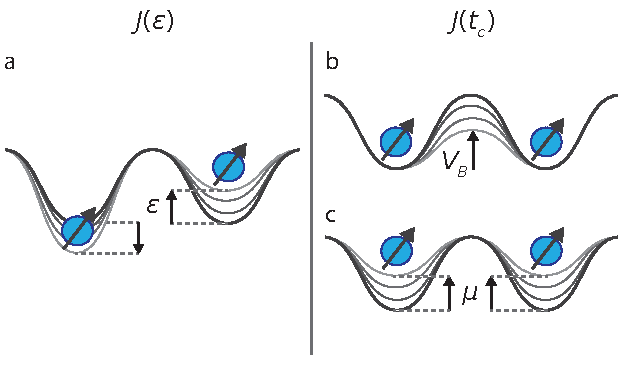
\includegraphics[width=\columnwidth]{figures/figure1_v4.pdf}
% \caption{\textbf{Replace this by the actual figures.} \textbf{(a)} Schematic. \textbf{(b)} Energy levels.}
% \label{fig:SchematicsDevice_And_Principle}
% \end{figure}
\section{Theory on single qubit operation}

Here we introduce the theory

\section{Experimental realization}

Here we start throwing data at the reader.
\\
\begin{figure}
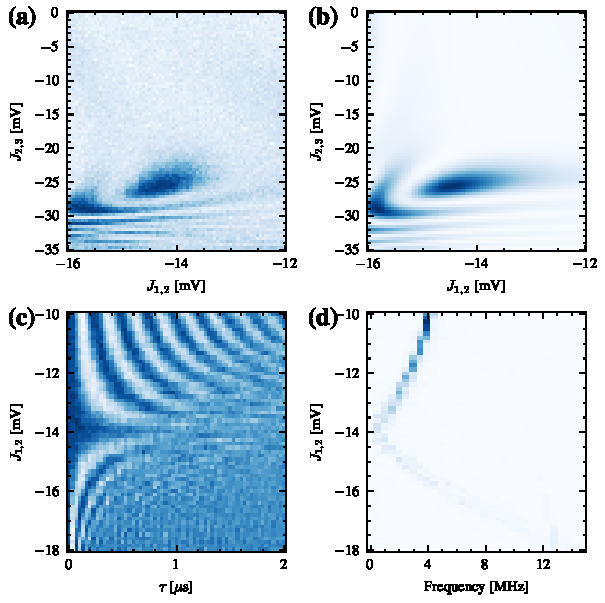
\includegraphics[width=\columnwidth]{figures/figure2/main.pdf}
\caption{\textbf{If you like it then you should throw data at it. TODO: this caption} \textbf{(a)} 2$\times$ 200 ns evolution time. Maybe add the pulses? \textbf{(b)} Simulated version of (a) using the parameters in S1. \textbf{(c)} Time evolution along $J_{2,3}$ after preparing a superposition using the calibrated values from (a) and projecting back unto z. \textbf{(d)} The fast fourier transform of c.}
\label{fig:Data_And_Numerics}
\end{figure}
% \begin{figure*}
% 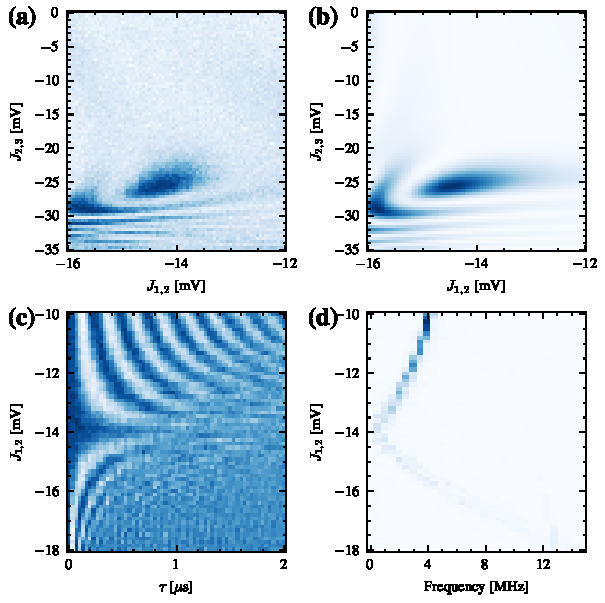
\includegraphics[width=\textwidth]{figures/figure2/main.pdf}
% \caption{\textbf{Also placeholder from different paper. If you like it then you should throw data at it.} \textbf{(a)} This should be meaningful text.}
% \label{fig:Data_And_Numerics}
% \end{figure*}

\section{Two-qubit gates}
Tess do your magic

\section{EO based shuttling architecture or smth}

Potential shuttling based architecture... TBD. Pretty drawings would be nice.

\section*{Methods}

At least we describe init and readout etc.

\section*{Acknowledgements}
We thank Sander de Snoo and Daan Bijl for continuous software development, and Olaf Benningshof for maintenance and support of the experimental setup.
\section*{Data Availability}
The code, analysis, and raw data supporting the findings of this study are openly available in a Zenodo repository: https://doi.org/somelink
\section*{Funding}

\DC{Any other funding we need to acknowledge from the theory side? TODO Ask Max/Stefano/Menno}

We acknowledge support by the Dutch Research Council through an NWO ENW grant and by the Dutch National Growth Fund (NGF), as part of the Quantum Delta NL programme. We acknowledge the European Union through ERC Starting Grant QUIST (850641) and through the IGNITE project of European Union’s Horizon Europe Framework Programme under grant agreement No. 101069515. This research was sponsored in part by the Army Research Office (ARO) under Award No. W911NF-23-1-0110. The views, conclusions, and recommendations contained in this document are those of the authors and are not necessarily endorsed nor should they be interpreted as representing the official policies, either expressed or implied, of the Army Research Office (ARO) or the U.S. Government. The
U.S. Government is authorized to reproduce and distribute reprints for Government purposes notwithstanding any copyright notation herein.


\section*{Competing Interest}
M.V. and G.S. are founding advisors of Groove Quantum BV, with M.V., and G.S. declaring equity interests. The remaining authors declare that they have no competing interests.

% \include{appendix}
\bibliography{references}% Produces the bibliography via BibTeX.

\end{document}
